\chapter{Modelling} \label{ch:model} 
Most of the modeling work has been performed on the data since there is no component meta-model to conform to. However, as a proof-of-concept exercise, it will be reported a conceptual example of how a model for this controller may look like.

\section{Data model}
Data modeling is partially supported in UBX in the sense that only a M0 and M1 model can be expressed. In the details, each data port defined in i-blocks and c-blocks have a predefined data-type; UBX only defines primitives data-types like integers and floating-points numbers and characters. Additional and composed types can be defined however; MicroBLX is not a mature project and therefore data-types are hand-written and stored in the \texttt{types} directory of the \texttt{ubx-control} project, but the idea behind data-types models is that an abstract meta-model should be instead be defined by the user, for example it is possible to do so using the JSon language, and leave to a tool-chain the dirty work of generating the language-specific headers files defining those data-types. Vice-versa it should be possible from the data instance to go back to its model, thats why all the data types defined have a meta data field that should be used to store the URI of the relative model.

\subsection{State data model}
The data meta-model of the state is a probability function representing an estimate of the real state of the system. This formulation is too general for being used with a Kalman filter, but may be useful if a more advanced estimator would be introduced, for example a particle filter. In this particular application we simply suppose to have a probability function representable with a Gaussian function, therefore a vector and a covariance matrix have been used to represent the state.\\
The state vector is a composition of the position vector and its first and second derivative and the orientation quaternion and its first and second derivatives (with a total size of 21 elements). The covariance matrix is accordingly a 21$\times$21 elements matrix.

\subsection{Sensor data model}
The sensor data model is similar to the state data model in the sense that is composed by a vector of arbitrary length (specified in an integer variable) and its covariance matrix. Please note that while the covariance matrix is a property of the sensor data only, the sensor model needed by the Kalman filter require the knowledge of both the state and the sensor data types, therefore it is specified as an input of the filter, not a property of the sensor data.

\subsection{Set-point and control action model}
The set-point and the control action can be represented using just a vectors: in this study case the set-point vector is a vector with the same structure used to represent the state, but no covariance matrix is necessary; the control action is a composition of the scalar thrust and the vector torque to be generated by the propellers.

\section{Filter model}
The meta-model of the extended Kalman filter is a Baysian estimator, multiple filters conforms to this type of filter like, for example, the particle filter. It is important to conform to the meta-model since conceptually it could be possible to have an automated model transformation tool able to select alternative filters to replace the original one and a supervisor able to switch the filter node on-line whenever necessary.\\
As example, think to have a controller that usually flies outdoor relaying on a GPS signal filtered by a Kalman filter for position estimation, but also embedded with a particle filter for indoor map-based navigation; it could be possible to have a software supervisor able to detect the feasibility of switching the GPS Kalman filter with the map-based particle filter and able to hot-swap those filters, thus allowing the vehicle to adapt the control system to the environment. For this to be possible, the supervisor should be able to perform model-transformation of both the data model and the filter model, thats why whenever this will be possible it will be necessary to have models of the components. A scheme in the following page shows conceptually the structure of the filter model.

\begin{figure}[ht]
\label{figmodel}
\begin{adjustbox}{addcode={\begin{minipage}{\width}}{\caption{The Kalman filter model and meta-model.}\end{minipage}},rotate=90,center}

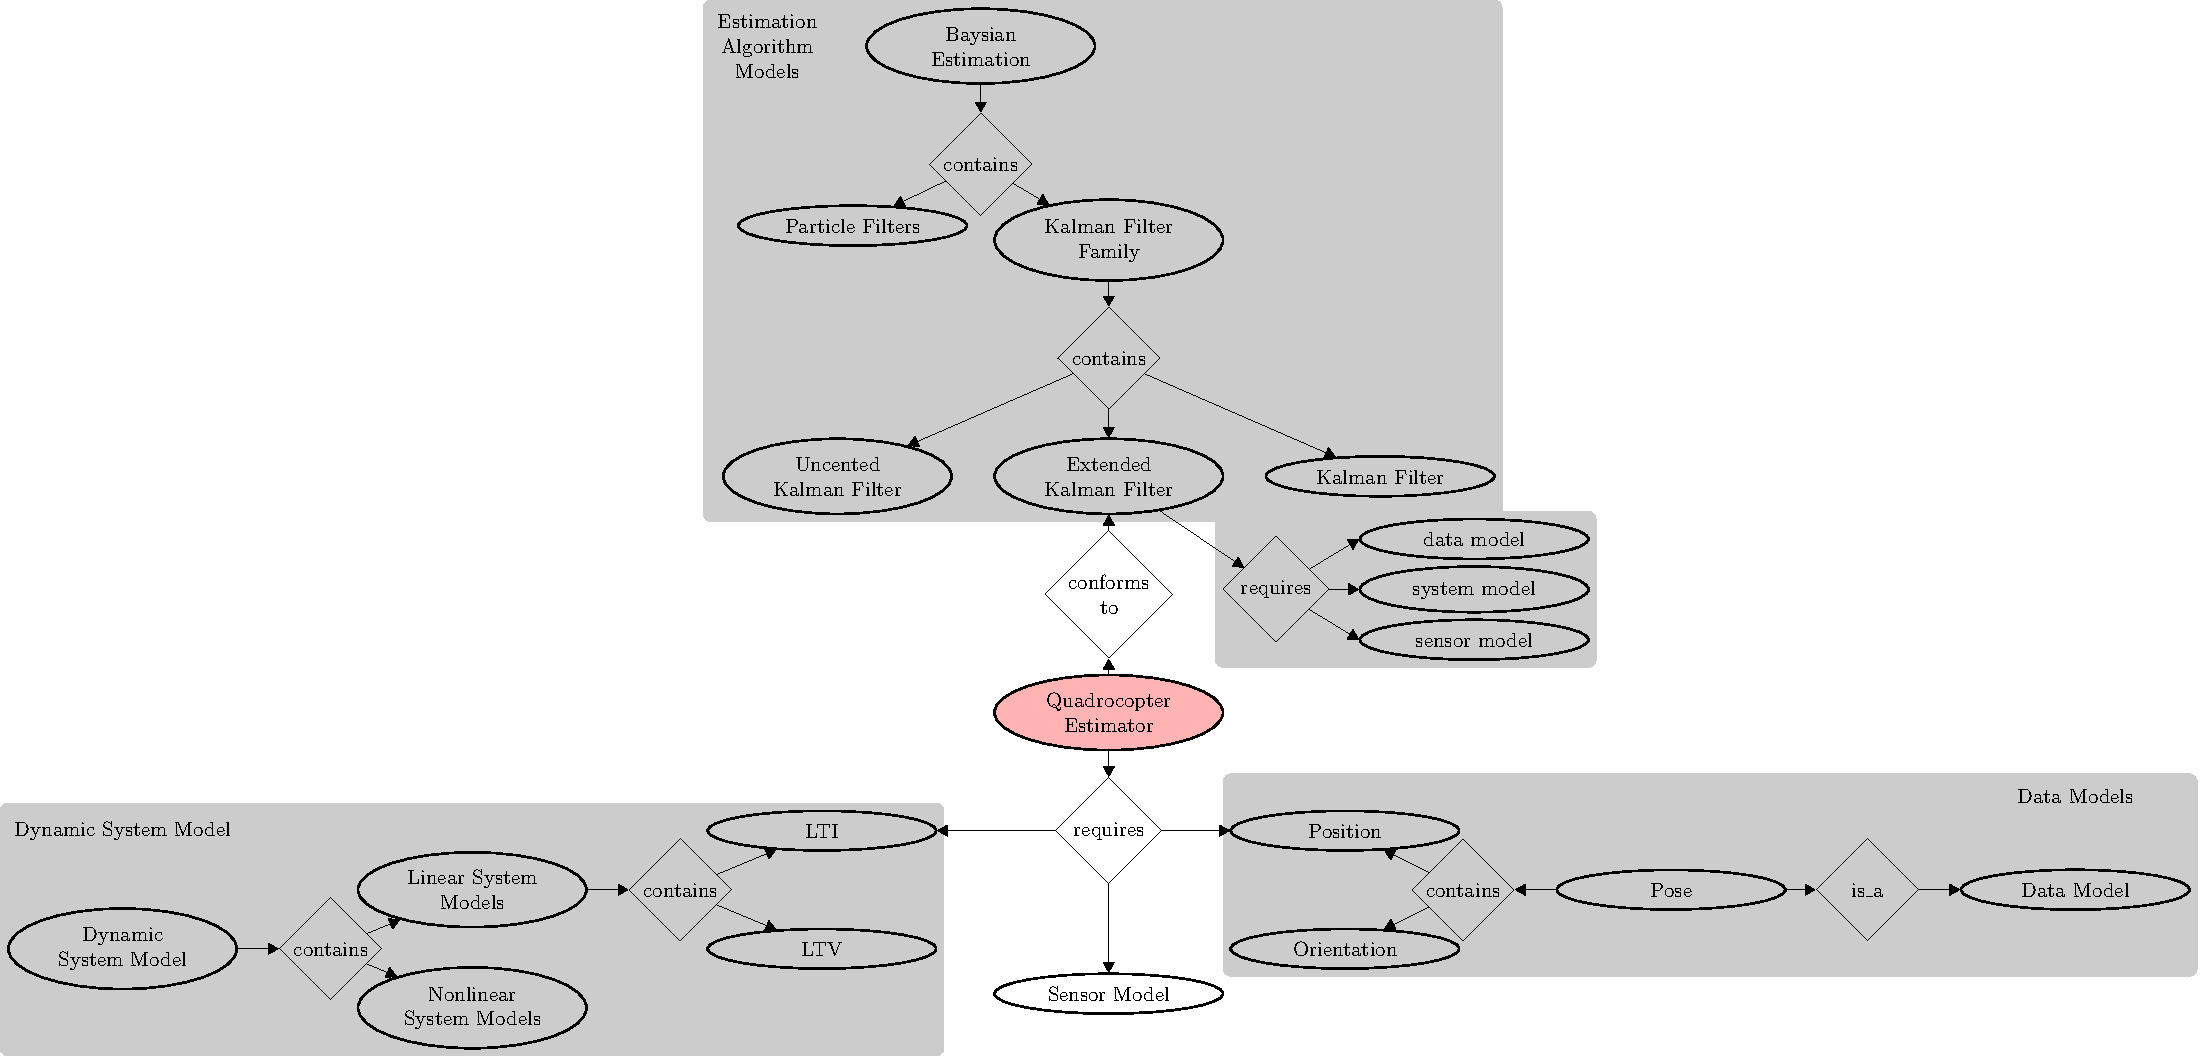
\includegraphics[scale=.6]{ekf_general}

\end{adjustbox}
\end{figure}

